%%=============================================================================
%% LaTeX sjabloon voor bachelorproef, HoGent Bedrijf en Organisatie
%% Opleiding Toegepaste Informatica
%%=============================================================================

\documentclass[fleqn,a4paper,12pt]{book}

%%=============================================================================
%% LaTeX sjabloon voor de bachelorproef, HoGent Bedrijf en Organisatie
%% Opleiding toegepaste informatica
%%
%% Structuur en algemene vormgeving. Meestal hoef je hier niets te wijzigen.
%%
%% Vormgeving gebaseerd op "The Legrand Orange Book", version 2.0 (9/2/15)
%% door Mathias Legrand (legrand.mathias@gmail.com) met aanpassingen door
%% Vel (vel@latextemplates.com). Het oorspronkelijke template is te vinden op
%% http://www.LaTeXTemplates.com
%%
%% Aanpassingen voor HoGent toegepaste informatica: 
%%   Bert Van Vreckem <bert.vanvreckem@hogent.be>
%% Licentie: 
%%   CC BY-NC-SA 3.0 (http://creativecommons.org/licenses/by-nc-sa/3.0/)
%%=============================================================================

%%-----------------------------------------------------------------------------
%% Packages
%%-----------------------------------------------------------------------------

\usepackage[top=3cm,bottom=3cm,left=3cm,right=3cm,headsep=10pt,a4paper]{geometry} % Page margins
\usepackage[utf8]{inputenc}  % Accenten gebruiken in tekst (vb. é ipv \'e)
\usepackage{amsfonts}        % AMS math packages: extra wiskundige
\usepackage{amsmath}         %   symbolen (o.a. getallen-
\usepackage{amssymb}         %   verzamelingen N, R, Z, Q, etc.)
\usepackage[english,dutch]{babel}    % Taalinstellingen: woordsplitsingen,
                             %  commando's voor speciale karakters
                             %  ("dutch" voor NL)
\usepackage{iflang}
\usepackage{eurosym}         % Euro-symbool €
\usepackage{geometry}
\usepackage{graphicx}        % Invoegen van tekeningen
\graphicspath{{img/}}       % Specifies the directory where pictures are stored
\usepackage{tikz}            % Required for drawing custom shapes
\usepackage[pdftex,bookmarks=true]{hyperref}
                             % PDF krijgt klikbare links & verwijzingen,
                             %  inhoudstafel
\usepackage{enumitem}        % Customize lists
\setlist{nolistsep}         % Reduce spacing between list items
\usepackage{listings}        % Broncode mooi opmaken
\usepackage{multirow}        % Tekst over verschillende cellen in tabellen
\usepackage{rotating}        % Tabellen en figuren roteren

\usepackage{booktabs}        % Required for nicer horizontal rules in tables

\usepackage{xcolor}          % Required for specifying colors by name
\definecolor{maincolor}{RGB}{0,147,208} % Define the main color used for 
                             % highlighting throughout the book
                             % 0, 147, 208 = officiële kleur HoGent FBO

% Paragraph style: no indent, add space between paragraphs
\setlength{\parindent}{0em}
\setlength{\parskip}{1em}

\usepackage{etoolbox}
\usepackage{titling} % Macros for title, author, etc
\usepackage{lipsum}          % Voor vultekst (lorem ipsum)

%----------------------------------------------------------------------------------------
%	FONTS
%----------------------------------------------------------------------------------------

\usepackage{avant} % Use the Avantgarde font for headings
%\usepackage{times} % Use the Times font for headings
\usepackage{mathptmx} % Use the Adobe Times Roman as the default text font together with math symbols from the Sym­bol, Chancery and Com­puter Modern fonts

\usepackage{microtype} % Slightly tweak font spacing for aesthetics
\usepackage[utf8]{inputenc} % Required for including letters with accents
\usepackage[T1]{fontenc} % Use 8-bit encoding that has 256 glyphs

%------------------------------------------------------------------------------
%	TITLE PAGE
%------------------------------------------------------------------------------

\newcommand{\inserttitlepage}{%
\begin{titlepage}
  \newgeometry{top=2cm,bottom=1.5cm,left=1.5cm,right=1.5cm}
  \begin{center}

    \begingroup
    \rmfamily
    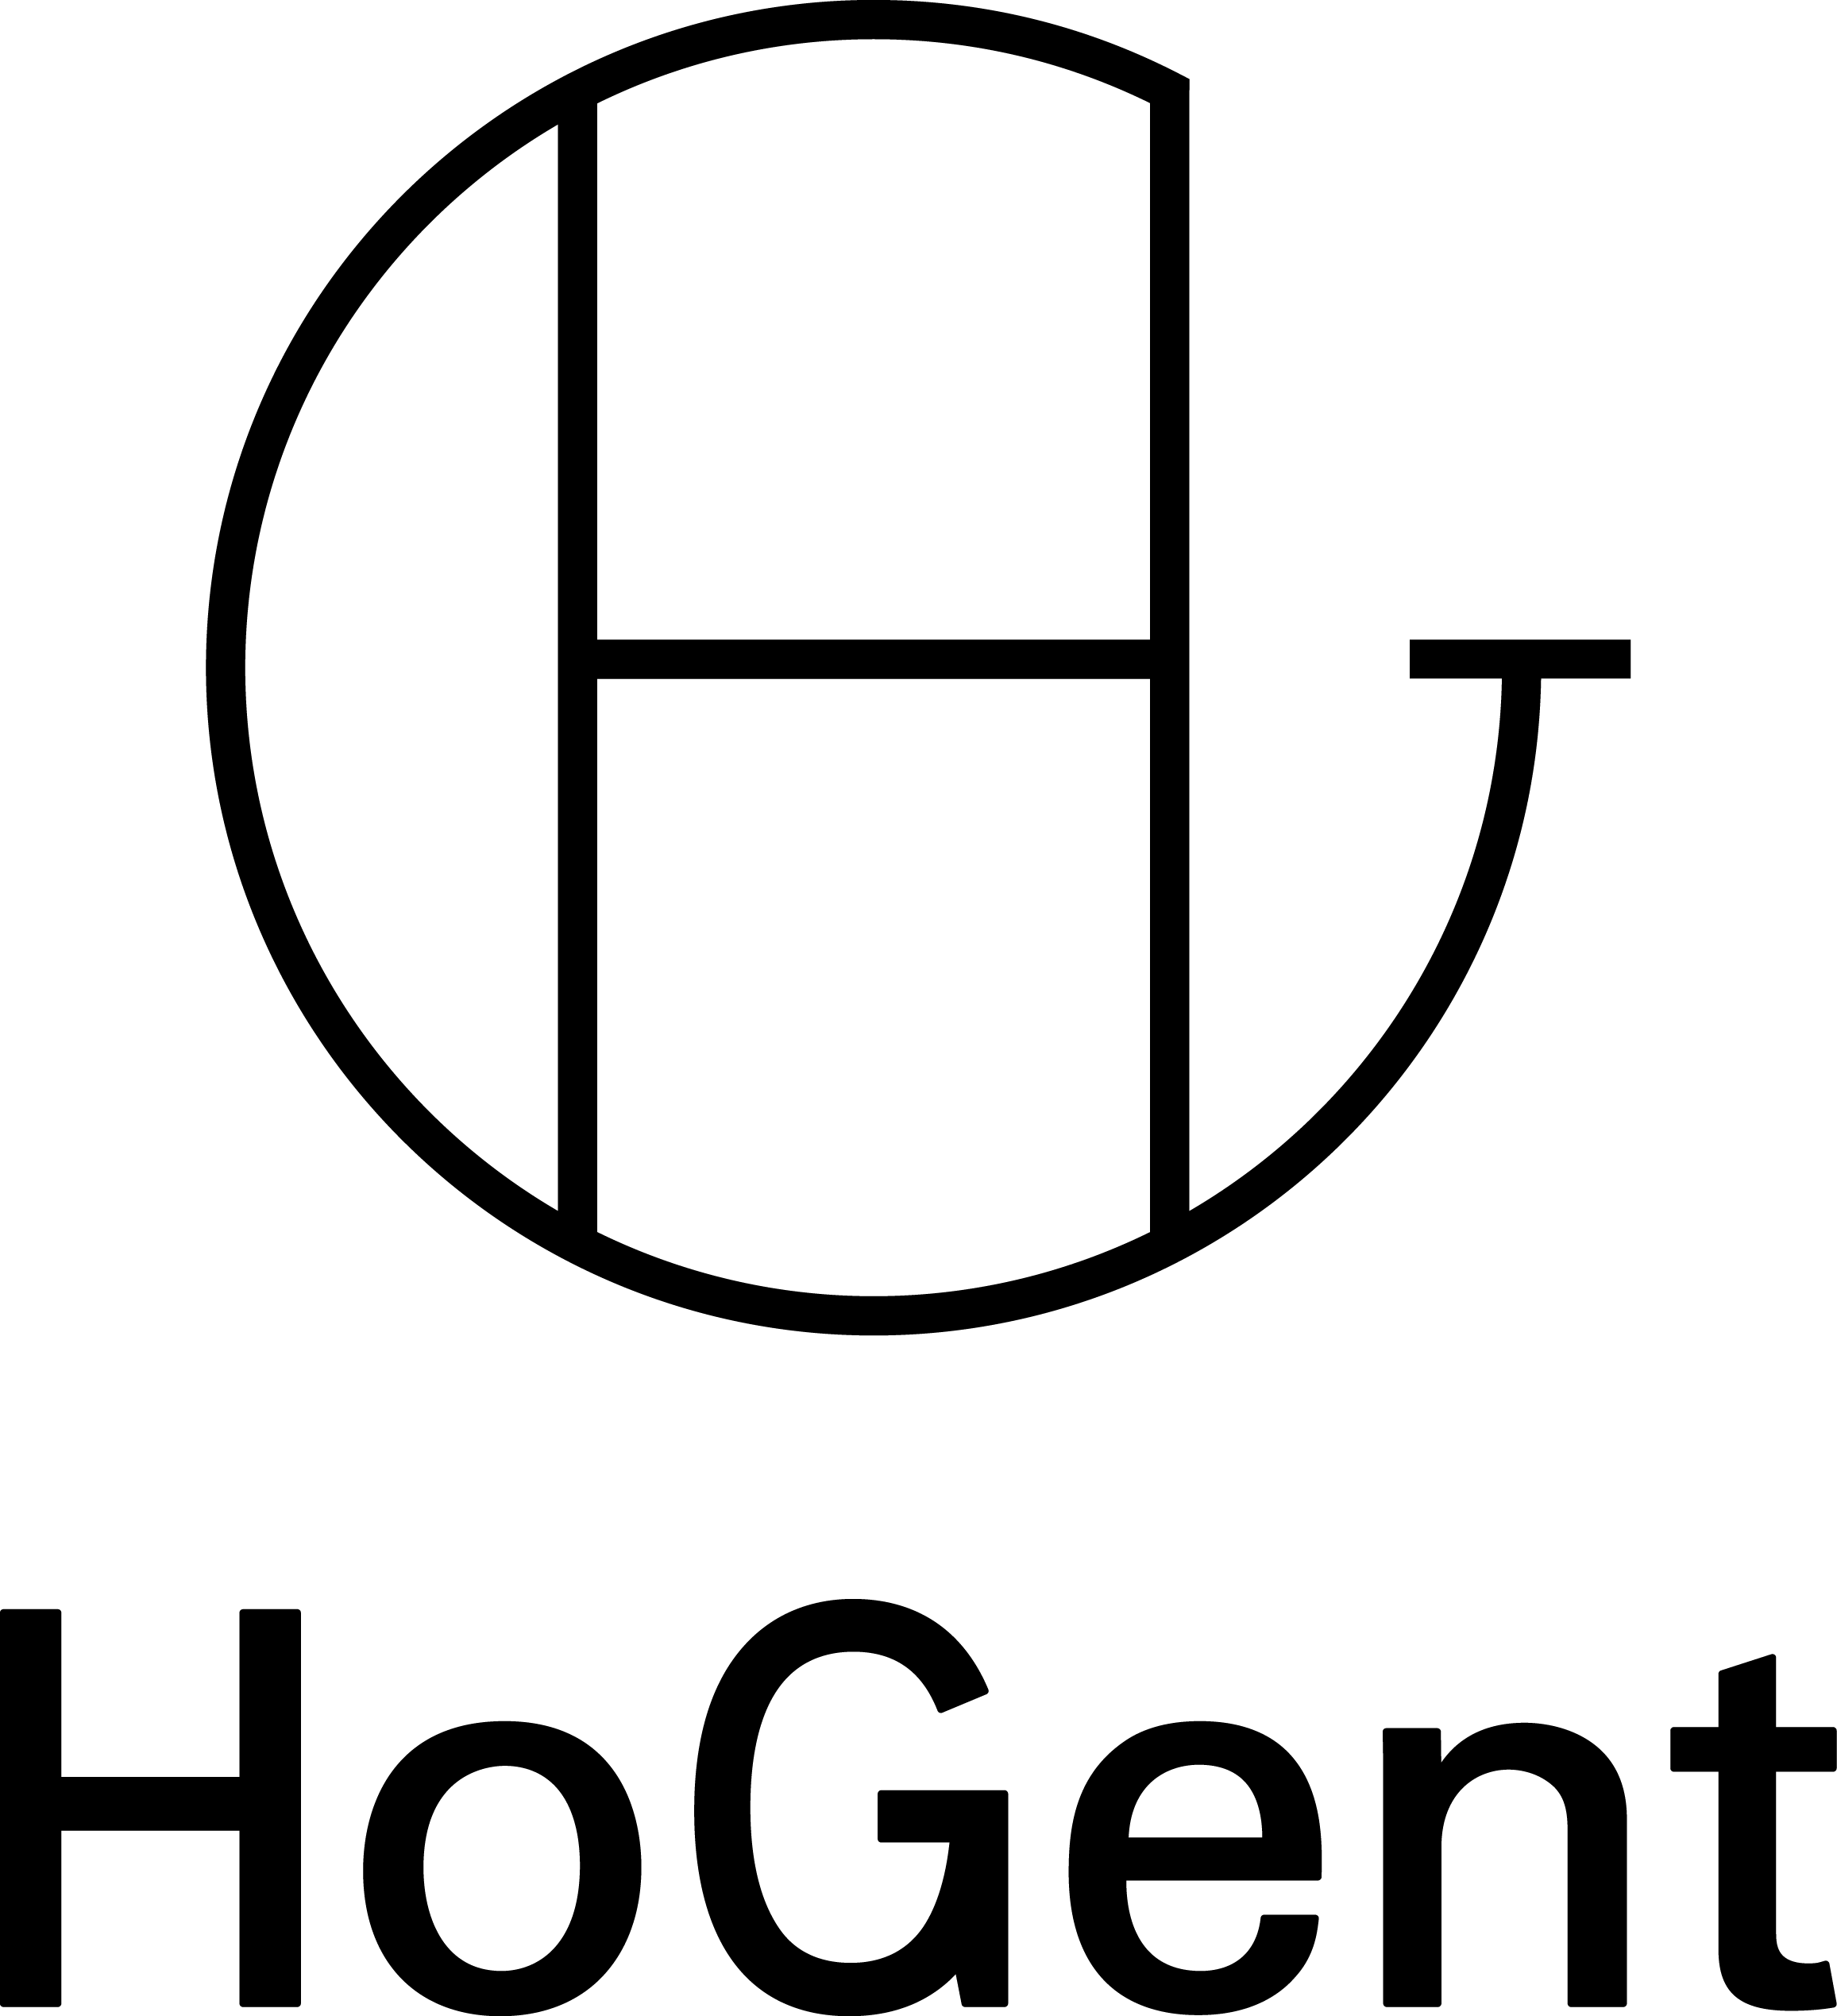
\includegraphics[width=2.5cm]{img/HG-beeldmerk-woordmerk}\\[.5cm]
    Faculteit Bedrijf en Organisatie\\[3cm]
    \titel
    \vfill
    \student\\[3.5cm]
    Scriptie voorgedragen tot het bekomen van de graad van\\professionele bachelor in de toegepaste informatica\\[2cm]
    Promotor:\\
    \promotor\\
    \ifdefempty{\copromotor}{\vspace{2.5cm}}{Co-promotor:\\\copromotor\\[2.5cm]}
    Instelling: \instelling\\[.5cm]
    Academiejaar: \academiejaar\\[.5cm]
    \ifcase \examenperiode \or Eerste \or Tweede \else Derde \fi examenperiode
    \endgroup

  \end{center}
  \restoregeometry
\end{titlepage}
  \emptypage
\begin{titlepage}
  \newgeometry{top=5.35cm,bottom=1.5cm,left=1.5cm,right=1.5cm}
  \begin{center}

    \begingroup
    \rmfamily
    \IfLanguageName{dutch}{Faculteit Bedrijf en Organisatie}{Faculty of Business and Information Management}\\[3cm]
    \titel
    \vfill
    \student\\[3.5cm]
    \IfLanguageName{dutch}{Scriptie voorgedragen tot het bekomen van de graad van\\professionele bachelor in de toegepaste informatica}{Thesis submitted in partial fulfilment of the requirements for the degree of\\professional bachelor of applied computer science}\\[2cm]
    Promotor:\\
    \promotor\\
    \ifdefempty{\copromotor}{\vspace{2.5cm}}{Co-promotor:\\\copromotor\\[2.5cm]}
    \IfLanguageName{dutch}{Instelling}{Institution}: \instelling\\[.5cm]
    \IfLanguageName{dutch}{Academiejaar}{Academic year}: \academiejaar\\[.5cm]
    \IfLanguageName{dutch}{%
    \ifcase \examenperiode \or Eerste \or Tweede \else Derde \fi examenperiode}{%
    \ifcase \examenperiode \or First \or Second \else Third \fi examination period}
    \endgroup

  \end{center}
  \restoregeometry
\end{titlepage}
}

%----------------------------------------------------------------------------------------
%	BIBLIOGRAPHY AND INDEX
%----------------------------------------------------------------------------------------

\usepackage[style=apa,backend=biber]{biblatex}
\usepackage{csquotes}
\DeclareLanguageMapping{dutch}{dutch-apa}
\addbibresource{bachproef-tin.bib} % BibTeX bibliography file
\addbibresource{./voorstel/voorstel.bib}
\defbibheading{bibempty}{}

\usepackage{calc} % For simpler calculation - used for spacing the index letter headings correctly
\usepackage{makeidx} % Required to make an index
\makeindex % Tells LaTeX to create the files required for indexing

%----------------------------------------------------------------------------------------
%	MAIN TABLE OF CONTENTS
%----------------------------------------------------------------------------------------

\usepackage{titletoc} % Required for manipulating the table of contents

\contentsmargin{0cm} % Removes the default margin

% Part text styling
\titlecontents{part}[0cm]
{\addvspace{20pt}\centering\large\bfseries}
{}
{}
{}

% Chapter text styling
\titlecontents{chapter}[1.25cm] % Indentation
{\addvspace{12pt}\large\sffamily\bfseries} % Spacing and font options for chapters
{\color{maincolor!60}\contentslabel[\Large\thecontentslabel]{1.25cm}\color{maincolor}} % Chapter number
{\color{maincolor}}
{\color{maincolor!60}\normalsize\;\titlerule*[.5pc]{.}\;\thecontentspage} % Page number

% Section text styling
\titlecontents{section}[1.25cm] % Indentation
{\addvspace{3pt}\sffamily\bfseries} % Spacing and font options for sections
{\contentslabel[\thecontentslabel]{1.25cm}} % Section number
{}
{\hfill\color{black}\thecontentspage} % Page number
[]

% Subsection text styling
\titlecontents{subsection}[1.25cm] % Indentation
{\addvspace{1pt}\sffamily\small} % Spacing and font options for subsections
{\contentslabel[\thecontentslabel]{1.25cm}} % Subsection number
{}
{\ \titlerule*[.5pc]{.}\;\thecontentspage} % Page number
[]

% List of figures
\titlecontents{figure}[0em]
{\addvspace{-5pt}\sffamily}
{\thecontentslabel\hspace*{1em}}
{}
{\ \titlerule*[.5pc]{.}\;\thecontentspage}
[]

% List of tables
\titlecontents{table}[0em]
{\addvspace{-5pt}\sffamily}
{\thecontentslabel\hspace*{1em}}
{}
{\ \titlerule*[.5pc]{.}\;\thecontentspage}
[]

%----------------------------------------------------------------------------------------
%	MINI TABLE OF CONTENTS IN PART HEADS
%----------------------------------------------------------------------------------------

% Chapter text styling
\titlecontents{lchapter}[0em] % Indenting
{\addvspace{15pt}\large\sffamily\bfseries} % Spacing and font options for chapters
{\color{maincolor}\contentslabel[\Large\thecontentslabel]{1.25cm}\color{maincolor}} % Chapter number
{}
{\color{maincolor}\normalsize\sffamily\bfseries\;\titlerule*[.5pc]{.}\;\thecontentspage} % Page number

% Section text styling
\titlecontents{lsection}[0em] % Indenting
{\sffamily\small} % Spacing and font options for sections
{\contentslabel[\thecontentslabel]{1.25cm}} % Section number
{}
{}

% Subsection text styling
\titlecontents{lsubsection}[.5em] % Indentation
{\normalfont\footnotesize\sffamily} % Font settings
{}
{}
{}

%----------------------------------------------------------------------------------------
%	PAGE HEADERS
%----------------------------------------------------------------------------------------

\usepackage{fancyhdr} % Required for header and footer configuration

\pagestyle{fancy}
\renewcommand{\chaptermark}[1]{\markboth{\sffamily\normalsize\bfseries\chaptername\ \thechapter.\ #1}{}} % Chapter text font settings
\renewcommand{\sectionmark}[1]{\markright{\sffamily\normalsize\thesection\hspace{5pt}#1}{}} % Section text font settings
\fancyhf{} \fancyhead[LE,RO]{\sffamily\normalsize\thepage} % Font setting for the page number in the header
\fancyhead[LO]{\rightmark} % Print the nearest section name on the left side of odd pages
\fancyhead[RE]{\leftmark} % Print the current chapter name on the right side of even pages
\renewcommand{\headrulewidth}{0.5pt} % Width of the rule under the header
\addtolength{\headheight}{2.5pt} % Increase the spacing around the header slightly
\renewcommand{\footrulewidth}{0pt} % Removes the rule in the footer
\fancypagestyle{plain}{\fancyhead{}\renewcommand{\headrulewidth}{0pt}} % Style for when a plain pagestyle is specified

% Removes the header from odd empty pages at the end of chapters
\makeatletter
\renewcommand{\cleardoublepage}{
\clearpage\ifodd\c@page\else
\hbox{}
\vspace*{\fill}
\thispagestyle{empty}
\newpage
\fi}

%----------------------------------------------------------------------------------------
%	THEOREM STYLES
%----------------------------------------------------------------------------------------

\usepackage{amsmath,amsfonts,amssymb,amsthm} % For math equations, theorems, symbols, etc

\newcommand{\intoo}[2]{\mathopen{]}#1\,;#2\mathclose{[}}
\newcommand{\ud}{\mathop{\mathrm{{}d}}\mathopen{}}
\newcommand{\intff}[2]{\mathopen{[}#1\,;#2\mathclose{]}}
\newtheorem{notation}{Notation}[chapter]

% Boxed/framed environments
\newtheoremstyle{maincolornumbox}% % Theorem style name
{0pt}% Space above
{0pt}% Space below
{\normalfont}% % Body font
{}% Indent amount
{\small\bf\sffamily\color{maincolor}}% % Theorem head font
{\;}% Punctuation after theorem head
{0.25em}% Space after theorem head
{\small\sffamily\color{maincolor}\thmname{#1}\nobreakspace\thmnumber{\@ifnotempty{#1}{}\@upn{#2}}% Theorem text (e.g. Theorem 2.1)
\thmnote{\nobreakspace\the\thm@notefont\sffamily\bfseries\color{black}---\nobreakspace#3.}} % Optional theorem note
\renewcommand{\qedsymbol}{$\blacksquare$}% Optional qed square

\newtheoremstyle{blacknumex}% Theorem style name
{5pt}% Space above
{5pt}% Space below
{\normalfont}% Body font
{} % Indent amount
{\small\bf\sffamily}% Theorem head font
{\;}% Punctuation after theorem head
{0.25em}% Space after theorem head
{\small\sffamily{\tiny\ensuremath{\blacksquare}}\nobreakspace\thmname{#1}\nobreakspace\thmnumber{\@ifnotempty{#1}{}\@upn{#2}}% Theorem text (e.g. Theorem 2.1)
\thmnote{\nobreakspace\the\thm@notefont\sffamily\bfseries---\nobreakspace#3.}}% Optional theorem note

\newtheoremstyle{blacknumbox} % Theorem style name
{0pt}% Space above
{0pt}% Space below
{\normalfont}% Body font
{}% Indent amount
{\small\bf\sffamily}% Theorem head font
{\;}% Punctuation after theorem head
{0.25em}% Space after theorem head
{\small\sffamily\thmname{#1}\nobreakspace\thmnumber{\@ifnotempty{#1}{}\@upn{#2}}% Theorem text (e.g. Theorem 2.1)
\thmnote{\nobreakspace\the\thm@notefont\sffamily\bfseries---\nobreakspace#3.}}% Optional theorem note

% Non-boxed/non-framed environments
\newtheoremstyle{maincolornum}% % Theorem style name
{5pt}% Space above
{5pt}% Space below
{\normalfont}% % Body font
{}% Indent amount
{\small\bf\sffamily\color{maincolor}}% % Theorem head font
{\;}% Punctuation after theorem head
{0.25em}% Space after theorem head
{\small\sffamily\color{maincolor}\thmname{#1}\nobreakspace\thmnumber{\@ifnotempty{#1}{}\@upn{#2}}% Theorem text (e.g. Theorem 2.1)
\thmnote{\nobreakspace\the\thm@notefont\sffamily\bfseries\color{black}---\nobreakspace#3.}} % Optional theorem note
\renewcommand{\qedsymbol}{$\blacksquare$}% Optional qed square
\makeatother

% Defines the theorem text style for each type of theorem to one of the three styles above
\newcounter{dummy}
\numberwithin{dummy}{section}
\theoremstyle{maincolornumbox}
\newtheorem{theoremeT}[dummy]{Theorem}
\newtheorem{problem}{Problem}[chapter]
\newtheorem{exerciseT}{Exercise}[chapter]
\theoremstyle{blacknumex}
\newtheorem{exampleT}{Example}[chapter]
\theoremstyle{blacknumbox}
\newtheorem{vocabulary}{Vocabulary}[chapter]
\newtheorem{definitionT}{Definition}[section]
\newtheorem{corollaryT}[dummy]{Corollary}
\theoremstyle{maincolornum}
\newtheorem{proposition}[dummy]{Proposition}

%----------------------------------------------------------------------------------------
%	DEFINITION OF COLORED BOXES
%----------------------------------------------------------------------------------------

\RequirePackage[framemethod=default]{mdframed} % Required for creating the theorem, definition, exercise and corollary boxes

% Theorem box
\newmdenv[skipabove=7pt,
skipbelow=7pt,
backgroundcolor=black!5,
linecolor=maincolor,
innerleftmargin=5pt,
innerrightmargin=5pt,
innertopmargin=5pt,
leftmargin=0cm,
rightmargin=0cm,
innerbottommargin=5pt]{tBox}

% Exercise box
\newmdenv[skipabove=7pt,
skipbelow=7pt,
rightline=false,
leftline=true,
topline=false,
bottomline=false,
backgroundcolor=maincolor!10,
linecolor=maincolor,
innerleftmargin=5pt,
innerrightmargin=5pt,
innertopmargin=5pt,
innerbottommargin=5pt,
leftmargin=0cm,
rightmargin=0cm,
linewidth=4pt]{eBox}

% Definition box
\newmdenv[skipabove=7pt,
skipbelow=7pt,
rightline=false,
leftline=true,
topline=false,
bottomline=false,
linecolor=maincolor,
innerleftmargin=5pt,
innerrightmargin=5pt,
innertopmargin=0pt,
leftmargin=0cm,
rightmargin=0cm,
linewidth=4pt,
innerbottommargin=0pt]{dBox}

% Corollary box
\newmdenv[skipabove=7pt,
skipbelow=7pt,
rightline=false,
leftline=true,
topline=false,
bottomline=false,
linecolor=gray,
backgroundcolor=black!5,
innerleftmargin=5pt,
innerrightmargin=5pt,
innertopmargin=5pt,
leftmargin=0cm,
rightmargin=0cm,
linewidth=4pt,
innerbottommargin=5pt]{cBox}

% Creates an environment for each type of theorem and assigns it a theorem text style from the "Theorem Styles" section above and a colored box from above
\newenvironment{theorem}{\begin{tBox}\begin{theoremeT}}{\end{theoremeT}\end{tBox}}
\newenvironment{exercise}{\begin{eBox}\begin{exerciseT}}{\hfill{\color{maincolor}\tiny\ensuremath{\blacksquare}}\end{exerciseT}\end{eBox}}
\newenvironment{definition}{\begin{dBox}\begin{definitionT}}{\end{definitionT}\end{dBox}}
\newenvironment{example}{\begin{exampleT}}{\hfill{\tiny\ensuremath{\blacksquare}}\end{exampleT}}
\newenvironment{corollary}{\begin{cBox}\begin{corollaryT}}{\end{corollaryT}\end{cBox}}

%----------------------------------------------------------------------------------------
%	REMARK ENVIRONMENT
%----------------------------------------------------------------------------------------

\newenvironment{remark}{\par\vspace{10pt}\small % Vertical white space above the remark and smaller font size
\begin{list}{}{
\leftmargin=35pt % Indentation on the left
\rightmargin=25pt}\item\ignorespaces % Indentation on the right
\makebox[-2.5pt]{\begin{tikzpicture}[overlay]
\node[draw=maincolor!60,line width=1pt,circle,fill=maincolor!25,font=\sffamily\bfseries,inner sep=2pt,outer sep=0pt] at (-15pt,0pt){\textcolor{maincolor}{R}};\end{tikzpicture}} % Orange R in a circle
\advance\baselineskip -1pt}{\end{list}\vskip5pt} % Tighter line spacing and white space after remark

%----------------------------------------------------------------------------------------
%	SECTION NUMBERING IN THE MARGIN
%----------------------------------------------------------------------------------------

\makeatletter
\renewcommand{\@seccntformat}[1]{\llap{\textcolor{maincolor}{\csname the#1\endcsname}\hspace{1em}}}
\renewcommand{\section}{\@startsection{section}{1}{\z@}
{-4ex \@plus -1ex \@minus -.4ex}
{1ex \@plus.2ex }
{\normalfont\large\sffamily\bfseries}}
\renewcommand{\subsection}{\@startsection {subsection}{2}{\z@}
{-3ex \@plus -0.1ex \@minus -.4ex}
{0.5ex \@plus.2ex }
{\normalfont\sffamily\bfseries}}
\renewcommand{\subsubsection}{\@startsection {subsubsection}{3}{\z@}
{-2ex \@plus -0.1ex \@minus -.2ex}
{.2ex \@plus.2ex }
{\normalfont\small\sffamily\bfseries}}
\renewcommand\paragraph{\@startsection{paragraph}{4}{\z@}
{-2ex \@plus-.2ex \@minus .2ex}
{.1ex}
{\normalfont\small\sffamily\bfseries}}

%----------------------------------------------------------------------------------------
%	PART HEADINGS
%----------------------------------------------------------------------------------------

% numbered part in the table of contents
\newcommand{\@mypartnumtocformat}[2]{%
\setlength\fboxsep{0pt}%
\noindent\colorbox{maincolor!20}{\strut\parbox[c][.7cm]{\ecart}{\color{maincolor!70}\Large\sffamily\bfseries\centering#1}}\hskip\esp\colorbox{maincolor!40}{\strut\parbox[c][.7cm]{\linewidth-\ecart-\esp}{\Large\sffamily\centering#2}}}%
%%%%%%%%%%%%%%%%%%%%%%%%%%%%%%%%%%
% unnumbered part in the table of contents
\newcommand{\@myparttocformat}[1]{%
\setlength\fboxsep{0pt}%
\noindent\colorbox{maincolor!40}{\strut\parbox[c][.7cm]{\linewidth}{\Large\sffamily\centering#1}}}%
%%%%%%%%%%%%%%%%%%%%%%%%%%%%%%%%%%
\newlength\esp
\setlength\esp{4pt}
\newlength\ecart
\setlength\ecart{1.2cm-\esp}
\newcommand{\thepartimage}{}%
\newcommand{\partimage}[1]{\renewcommand{\thepartimage}{#1}}%
\def\@part[#1]#2{%
\ifnum \c@secnumdepth >-2\relax%
\refstepcounter{part}%
\addcontentsline{toc}{part}{\texorpdfstring{\protect\@mypartnumtocformat{\thepart}{#1}}{\partname~\thepart\ ---\ #1}}
\else%
\addcontentsline{toc}{part}{\texorpdfstring{\protect\@myparttocformat{#1}}{#1}}%
\fi%
\startcontents%
\markboth{}{}%
{\thispagestyle{empty}%
\begin{tikzpicture}[remember picture,overlay]%
\node at (current page.north west){\begin{tikzpicture}[remember picture,overlay]%
\fill[maincolor!20](0cm,0cm) rectangle (\paperwidth,-\paperheight);
\node[anchor=north] at (4cm,-3.25cm){\color{maincolor!40}\fontsize{220}{100}\sffamily\bfseries\@Roman\c@part};
\node[anchor=south east] at (\paperwidth-1cm,-\paperheight+1cm){\parbox[t][][t]{8.5cm}{
\printcontents{l}{0}{\setcounter{tocdepth}{1}}%
}};
\node[anchor=north east] at (\paperwidth-1.5cm,-3.25cm){\parbox[t][][t]{15cm}{\strut\raggedleft\color{white}\fontsize{30}{30}\sffamily\bfseries#2}};
\end{tikzpicture}};
\end{tikzpicture}}%
\@endpart}
\def\@spart#1{%
\startcontents%
\phantomsection
{\thispagestyle{empty}%
\begin{tikzpicture}[remember picture,overlay]%
\node at (current page.north west){\begin{tikzpicture}[remember picture,overlay]%
\fill[maincolor!20](0cm,0cm) rectangle (\paperwidth,-\paperheight);
\node[anchor=north east] at (\paperwidth-1.5cm,-3.25cm){\parbox[t][][t]{15cm}{\strut\raggedleft\color{white}\fontsize{30}{30}\sffamily\bfseries#1}};
\end{tikzpicture}};
\end{tikzpicture}}
\addcontentsline{toc}{part}{\texorpdfstring{%
\setlength\fboxsep{0pt}%
\noindent\protect\colorbox{maincolor!40}{\strut\protect\parbox[c][.7cm]{\linewidth}{\Large\sffamily\protect\centering #1\quad\mbox{}}}}{#1}}%
\@endpart}
\def\@endpart{\vfil\newpage
\if@twoside
\if@openright
\null
\thispagestyle{empty}%
\newpage
\fi
\fi
\if@tempswa
\twocolumn
\fi}

%----------------------------------------------------------------------------------------
%	CHAPTER HEADINGS
%----------------------------------------------------------------------------------------

% A switch to conditionally include a picture, implemented by  Christian Hupfer
\newif\ifusechapterimage
\usechapterimagetrue
\newcommand{\thechapterimage}{}%
\newcommand{\chapterimage}[1]{\ifusechapterimage\renewcommand{\thechapterimage}{#1}\fi}%
\def\@makechapterhead#1{%
{\parindent \z@ \raggedright \normalfont
\ifnum \c@secnumdepth >\m@ne
\if@mainmatter
\begin{tikzpicture}[remember picture,overlay]
\node at (current page.north west)
{\begin{tikzpicture}[remember picture,overlay]
\node[anchor=north west,inner sep=0pt] at (0,0) {\ifusechapterimage\includegraphics[width=\paperwidth]{\thechapterimage}\fi};
\draw[anchor=west] (\Gm@lmargin,-9cm) node [line width=2pt,rounded corners=15pt,draw=maincolor,fill=white,fill opacity=0.5,inner sep=15pt]{\strut\makebox[22cm]{}};
\draw[anchor=west] (\Gm@lmargin+.3cm,-9cm) node {\huge\sffamily\bfseries\color{black}\thechapter. #1\strut};
\end{tikzpicture}};
\end{tikzpicture}
\else
\begin{tikzpicture}[remember picture,overlay]
\node at (current page.north west)
{\begin{tikzpicture}[remember picture,overlay]
\node[anchor=north west,inner sep=0pt] at (0,0) {\ifusechapterimage\includegraphics[width=\paperwidth]{\thechapterimage}\fi};
\draw[anchor=west] (\Gm@lmargin,-9cm) node [line width=2pt,rounded corners=15pt,draw=maincolor,fill=white,fill opacity=0.5,inner sep=15pt]{\strut\makebox[22cm]{}};
\draw[anchor=west] (\Gm@lmargin+.3cm,-9cm) node {\huge\sffamily\bfseries\color{black}#1\strut};
\end{tikzpicture}};
\end{tikzpicture}
\fi\fi\par\vspace*{270\p@}}}

%-------------------------------------------

\def\@makeschapterhead#1{%
\begin{tikzpicture}[remember picture,overlay]
\node at (current page.north west)
{\begin{tikzpicture}[remember picture,overlay]
\node[anchor=north west,inner sep=0pt] at (0,0) {\ifusechapterimage\includegraphics[width=\paperwidth]{\thechapterimage}\fi};
\draw[anchor=west] (\Gm@lmargin,-9cm) node [line width=2pt,rounded corners=15pt,draw=maincolor,fill=white,fill opacity=0.5,inner sep=15pt]{\strut\makebox[22cm]{}};
\draw[anchor=west] (\Gm@lmargin+.3cm,-9cm) node {\huge\sffamily\bfseries\color{black}#1\strut};
\end{tikzpicture}};
\end{tikzpicture}
\par\vspace*{270\p@}}
\makeatother

%----------------------------------------------------------------------------------------
%	HYPERLINKS IN THE DOCUMENTS
%----------------------------------------------------------------------------------------

\usepackage{hyperref}
\hypersetup{hidelinks,backref=true,pagebackref=true,hyperindex=true,colorlinks=false,breaklinks=true,urlcolor= maincolor,bookmarks=true,bookmarksopen=false,pdftitle={Title},pdfauthor={Author}}
\usepackage{bookmark}
\bookmarksetup{
open,
numbered,
addtohook={%
\ifnum\bookmarkget{level}=0 % chapter
\bookmarksetup{bold}%
\fi
\ifnum\bookmarkget{level}=-1 % part
\bookmarksetup{color=maincolor,bold}%
\fi
}
}

%----------------------------------------------------------------------------------------
%	Java source code
%----------------------------------------------------------------------------------------

% Commando voor invoegen Java-broncodebestanden (dank aan Niels Corneille)
% Gebruik:
%   \codefragment{source/MijnKlasse.java}{Uitleg bij de code}
%
% Je kan dit aanpassen aan de taal die je zelf het meeste gebruikt in je
% bachelorproef.
\newcommand{\codefragment}[2]{ \lstset{%
  language=java,
  breaklines=true,
  float=th,
  caption={#2},
  basicstyle=\scriptsize,
  frame=single,
  extendedchars=\true
}
\lstinputlisting{#1}}

% Leeg blad
\newcommand{\emptypage}{%
\newpage
\thispagestyle{empty}
\mbox{}
\newpage
}


%%---------- Documenteigenschappen --------------------------------------------
%% TODO: Vul dit aan met je eigen info:

% Je eigen naam
\newcommand{\student}{Preben Leroy}

% De naam van je promotor (lector van de opleiding)
\newcommand{\promotor}{Steven Van Impe}

% De naam van je co-promotor. Als je promotor ook je opdrachtgever is en je
% dus ook inhoudelijk begeleidt (en enkel dan!), mag je dit leeg laten.
\newcommand{\copromotor}{Karel Serruys}

% Indien je bachelorproef in opdracht van/in samenwerking met een bedrijf of
% externe organisatie geschreven is, geef je hier de naam. Zoniet laat je dit
% zoals het is.
\newcommand{\instelling}{---}

% De titel van het rapport/bachelorproef
\newcommand{\titel}{Delaware Consulting (Gent)}

% Datum van indienen (gebruik telkens de deadline, ook al geef je eerder af)
\newcommand{\datum}{28 mei 2018}

% Academiejaar
\newcommand{\academiejaar}{2017-2018}

% Examenperiode
%  - 1e semester = 1e examenperiode => 1
%  - 2e semester = 2e examenperiode => 2
%  - tweede zit  = 3e examenperiode => 3
\newcommand{\examenperiode}{2}

%%=============================================================================
%% Inhoud document
%%=============================================================================

\begin{document}

%---------- Taalselectie ------------------------------------------------------
% Als je je bachelorproef in het Engels schrijft, haal dan onderstaande regel
% uit commentaar. Let op: de tekst op de voorkaft blijft in het Nederlands, en
% dat is ook de bedoeling!

%\selectlanguage{english}

%---------- Titelblad ---------------------------------------------------------
\inserttitlepage

%---------- Samenvatting, voorwoord -------------------------------------------
\usechapterimagefalse
%%=============================================================================
%% Voorwoord
%%=============================================================================

\chapter*{Woord vooraf}
\label{ch:voorwoord}

%% TODO:
%% Het voorwoord is het enige deel van de bachelorproef waar je vanuit je
%% eigen standpunt (``ik-vorm'') mag schrijven. Je kan hier bv. motiveren
%% waarom jij het onderwerp wil bespreken.
%% Vergeet ook niet te bedanken wie je geholpen/gesteund/... heeft
\begin{flushright}
	\textit{Mei, 2018}
\end{flushright}

Deze bachelorproef dient als sluitstuk van mijn driejarige opleiding Toegepaste Informatica aan Hogeschool Gent. Hiermee wil ik aantonen dat ik op een kritische manier een onderzoek kan uitvoeren naar een nog niet zo evident onderwerp in de IT. De IT-wereld is een wereld die altijd in verandering is. Daarom is het belangrijk dat men altijd op een kritische manier nieuwe technologieën onderzoekt.

Het onderzoek dat ik zal uitvoeren in deze bachelorproef heeft te maken met artificiële intelligentie. AI speelt een belangrijke rol in ons dagelijks leven. In de toekomst zal het zelfs nog belangrijker zijn dan vandaag. Denk hierbij maar aan zelfrijdende auto's of automatische stofzuigers en dergelijke. 

Door toedoen van artificiële intelligentie zal ook onze maatschappij grondig veranderen. Vele jobs zullen hierdoor verdwijnen. Ook in de wereld van de IT. Daarom vond ik het belangrijk hiernaar onderzoek te doen. Bestaat er een kans dat AI het werk van een IT'er gaat overnemen, in het bijzonder het werk van een programmeur? Dit ga ik trachten te onderzoeken. 

Graag zou ik mijn promotor, de heer Steven Van Impe, en mijn co-promotor, de heer Karel Serruys, willen bedanken om mij met raad en daad bij te staan doorheen dit proces. Terwijl de heer Van Impe mij vooral op technisch vlak ondersteunde, hielp de heer Karel Serruys mij op inhoudelijk vlak. Hij was degene die mij in de juiste richting dreef voor het uitvoeren van dit onderzoek.

\break
Daarnaast zou ik graag mijn ouders bedanken om mij de afgelopen drie jaar te ondersteunen, zeker op momenten wanneer het moeilijk ging. Ook al weten of begrijpen ze niet waarmee ik bezig ben, toch probeerden zij mij bij te staan. Hierbij zou ik mij ook willen excuseren wanneer ik mij de afgelopen drie jaar misschien wat irritant gedraagde wanneer het wat moeilijker ging. 

Ik wens iedere lezer veel leesplezier bij het lezen van deze bachelorproef.

\begin{flushright}
	\textit{Preben Leroy \\
		Bachelor Toegepaste Informatica, keuzepakket Mobile Applicaties \\
		Hogeschool Gent \\
		Academiejaar 2017-2018}
\end{flushright}
%%=============================================================================
%% Samenvatting
%%=============================================================================

% TODO: De "abstract" of samenvatting is een kernachtige (~ 1 blz. voor een
% thesis) synthese van het document.
%
% Deze aspecten moeten zeker aan bod komen:
% - Context: waarom is dit werk belangrijk?
% - Nood: waarom moest dit onderzocht worden?
% - Taak: wat heb je precies gedaan?
% - Object: wat staat in dit document geschreven?
% - Resultaat: wat was het resultaat?
% - Conclusie: wat is/zijn de belangrijkste conclusie(s)?
% - Perspectief: blijven er nog vragen open die in de toekomst nog kunnen
%    onderzocht worden? Wat is een mogelijk vervolg voor jouw onderzoek?
%
% LET OP! Een samenvatting is GEEN voorwoord!

%%---------- Nederlandse samenvatting -----------------------------------------
%
% TODO: Als je je bachelorproef in het Engels schrijft, moet je eerst een
% Nederlandse samenvatting invoegen. Haal daarvoor onderstaande code uit
% commentaar.
% Wie zijn bachelorproef in het Nederlands schrijft, kan dit negeren, de inhoud
% wordt niet in het document ingevoegd.

\IfLanguageName{english}{%
\selectlanguage{dutch}
\chapter*{Samenvatting}

\selectlanguage{english}
}{}

%%---------- Samenvatting -----------------------------------------------------
% De samenvatting in de hoofdtaal van het document

\chapter*{\IfLanguageName{dutch}{Samenvatting}{Abstract}}

Deze bachelorproef staat in het teken van artificiële intelligentie en de mogelijkheid om door middel van AI en natuurlijke taal programmeercode te laten genereren. Eerst en vooral wordt er uitleg verschaft van wat de achterliggende technieken zijn die gebruikt worden bij de generatie, om dan over te gaan naar een aantal reeds bestaande voorbeelden. Het is belangrijk dat de mogelijkheid tot het genereren van code door middel van AI wordt onderzocht. Tegenwoordig neemt artificiële intelligentie heel wat van onze taken over, denk hierbij maar aan automatische stofzuigers, zelfrijdende auto's en zelfs spraakherkenning op smartphones.

Artificiële intelligentie is nu al een belangrijk issue in onze maatschappij, maar dit zal nog belangrijker worden dan eerst gedacht. Zo worden er in een artikel (\textcite{Gartner}) een aantal voorspellingen gedaan over de toekomst. Hierin werd onder andere besproken dat de technische wereld grondig zou veranderen door de groei aan toepassingen waarbij AI gebruikt worden. Gartner vertelt bijvoorbeeld dat tegen 2022 slimme technologieën en robots allerhande taken zouden overnemen in de geneeskunde en in de IT. Dat laatste is natuurlijk belangrijk voor de IT'ers van nu en van de toekomst. Zou artificiële intelligentie bijvoorbeeld het werk van een programmeur kunnen overnemen in de toekomst? Zouden wij, als programmeurs, in de toekomst geen werk meer hebben? In deze bachelorproef wordt hier getracht een antwoord op te bieden. 

Er werd eerst een studie gedaan naar reeds bestaande technologieën, zoals de Microsoft DeepCoder en Google's AutoML. Ook werden er een aantal concretere cases besproken, zoals Seq2SQL en SQLNet. Het werd al snel duidelijk dat de overgrote meerderheid van de cases de generatie van SQL-query's behandelden. De reden hiervoor is dat de syntax van de programmeertaal SQL grotendeels gelijkaardig is aan de natuurlijke taal. Zo'n programmeertaal behoort tot de vierde generatie programmeertalen.

Naast een uitgebreide literatuurstudie over deze cases, werden er dan ook enkele uitgetest. Hiervoor werd gekozen voor de Seq2SQL-case, voor de SQLNet-case en ook voor WikiSQL. Iedere case wordt eerst nog eens kort besproken van wat het precies is, om dan over te gaan naar de opbouw van het algoritme en de nodige scripts. Uiteindelijk werd er getracht deze scripts uit te voeren en resultaten te bekomen om zo een mogelijke conclusie te bekomen.

-- Resultaten --

-- Conclusie --

Artificiële intelligentie is een recente wetenschap. Alles veranderd met de tijd. Natuurlijk is het mogelijk om in de toekomst nog verder onderzoek te doen naar het gebruik van artificiële intelligentie in de wereld van de IT. Dit reeds gevoerde onderzoek zou mogelijks in de toekomst misschien wel andere resultaten kunnen opleveren dan de reeds bekomen resultaten. 


%---------- Inhoudstafel ------------------------------------------------------
\pagestyle{empty} % No headers
\tableofcontents % Print the table of contents itself
\cleardoublepage % Forces the first chapter to start on an odd page so it's on the right
\pagestyle{fancy} % Print headers again

%---------- Lijst figuren, afkortingen, ... -----------------------------------

% Indien gewenst kan je hier een lijst van figuren/tabellen opgeven. Geef in
% dat geval je figuren/tabellen altijd een korte beschrijving:
%
%  \caption[korte beschrijving]{uitgebreide beschrijving}

\listoffigures
\listoftables

% Als je een lijst van afkortingen of termen wil toevoegen, dan hoort die
% hier thuis. Gebruik bijvoorbeeld de ``glossaries'' package.
% https://www.sharelatex.com/learn/Glossaries

%%---------- Kern -------------------------------------------------------------

%%=============================================================================
%% Inleiding
%%=============================================================================

\chapter*{Inleiding}
\label{ch:inleiding}

Artificiële intelligentie is reeds een hot topic in onze maatschappij. Tegenwoordig kan het overal in toegepast worden. Zo wordt het gebruikt in een aantal toepassingen zoals gezichtsherkenning, zelfrijdende auto’s, … . Maar wordt het ook voor andere toepassingen de standaard?

In dit onderzoek gaat het niet over het algemene aspect dat artificiële intelligentie alles zou overnemen. Hier gaan we dieper in op het feit dat AI de ICT drastisch kan veranderen. Zeker voor de programmeurs onder de ICT’ers. Daarom wordt in deze Bachelorproef een onderzoek gedaan naar de mogelijkheid om code te laten genereren door middel van AI vanuit natuurlijke taal. 

De vragen die je aan het systeem zou stellen, moeten wel een functioneel karakter hebben. De functionele specificaties van het te bouwen programma moeten in de vraag voorkomen. Bij deze specificaties wordt er helder beschreven waaraan het programma moet voldoen. Hoe duidelijker de vraag aan het systeem, hoe gedetailleerder het systeem code zou kunnen schrijven.  

\section{Probleemstelling}
\label{sec:probleemstelling}

In het artikel van \textcite{Gartner} worden er een aantal voorspellingen van de toekomst gedaan. Volgens het artikel zou de technologische wereld grondig veranderen door de groei van het toepassen van artificiële intelligentie.  Gartner voorspelt onder ander dat in 2022 slimme technologieën en robots taken kunnen overnemen in de geneeskunde en in de IT. Dit zijn taken van meestal hoog opgeleide mensen.

Volgens Gartner zullen bedrijven in de toekomst hun bedrijfsstrategieën moeten aanpassen. Artificiële intelligentie zullen in de toekomst meer en meer complexere zaken uitvoeren. De effecten die AI in de toekomst zou hebben in bedrijven, hangt af van sector tot sector. Daarnaast moet er verder ook rekening gehouden worden met de klanten van het bedrijf. 

Ook in de IT wordt AI als maar belangrijker. Gartner verwacht dat artificiële intelligentie de routine functies van IT-organisaties zal gaan vervangen. Dit zal voornamelijk  gebeuren langs de operationele kant. Sommige functies zullen verdwijnen, AI neemt deze dan over en zal de werking ervan nog verbeteren. Dit onderzoek zoekt antwoorden op vragen die hierbij aansluiten. Is het bijvoorbeeld mogelijk om ui natuurlijke taal iets functioneel te bouwen in de IT? 

Voor mezelf lijkt dit onderzoek in eerste plaats bruikbaar voor softwareontwikkeling. Je kan zo de vraag stellen of het weldegelijk toepasbaar is op alle programmeertalen die tegenwoordig gebruikt worden. 

Niet alleen pure softwarebedrijven kunnen de vruchten plukken van dit onderzoek, maar ook bedrijven die zich vooral toeleggen om databank transacties, of die allerlei queries stuurt om data op te halen in een databank. Is het bijvoorbeeld mogelijk om gewoon te kunnen zeggen tegen een databank: “Geef eens de afrekeningen van de afgelopen 12 maanden van klant y”. 

Toen ik een onderwerp zocht voor deze Bachelorproef, nam ik contact op met mijn stagebedrijf (delaware) of niemand daar tips kon geven. Ik wou iets doen rond AI en rond programmeren. Mijn huidige co-promotor gaf mij dit als mogelijk onderwerp. In het bedrijf wordt er veel gebruik gemaakt van de SAP/4HANA-databank. Denk hierbij ook aan bovenstaand voorbeeld, is het ook mogelijk om met deze databank in natuurlijke taal te kunnen communiceren? Tijdens dit onderzoek zal ik hierop een antwoord proberen bieden.

\section{Onderzoeksvraag}
\label{sec:onderzoeksvraag}

Dit onderzoek gaat over het gebruik van artificiële intelligentie in de IT. Vooral voor programmeurs kan dit enige gevolgen hebben. De algemene vraag die door programmeurs kan gesteld worden, is of het mogelijk is om door middel van AI code te laten genereren. Specifiek genereren op basis vaan natuurlijke taal. 

Naast deze eerder makkelijke vraag, kunnen ook de volgende echte onderzoeksvragen gesteld worden:
\begin{itemize}
	\item Voor welke programmeertalen is het nu al mogelijk om code te genereren vanuit natuurlijke taal (door middel van AI)?
	\item Aan wat moet een algoritme voldoen om de code te kunnen genereren?
	\begin{itemize}
		\item Zijn er voor- en/of nadelen verbonden aan de generatie indien het op die bepaalde manier gebeurd?
		\item Zijn er eventuele beperkingen gebonden om een werkend algoritme te verkrijgen?
	\end{itemize}
	\item Hoe worden zo'n algoritmen in de praktijk uitgevoerd?
	\begin{itemize}
		\item Zijn er voor- en/of nadelen verbonden aan de generatie indien het op die bepaalde manier gebeurd?
		\item Zijn er eventuele beperkingen gebonden om een algoritme werkende te krijgen wanneer de dataset een bepaalde configuratie heeft?
	\end{itemize}
	\item Aan wat dient een dataset te voldoen om het mogelijk te maken om bepaalde algoritmes erop toe te kunnen passen?
\end{itemize}

\section{Onderzoeksdoelstelling}
\label{sec:onderzoeksdoelstelling}

Wat is het beoogde resultaat van je bachelorproef? Wat zijn de criteria voor succes? Beschrijf die zo concreet mogelijk.

\section{Opzet van deze bachelorproef}
\label{sec:opzet-bachelorproef}

Volgende onderdelen kan u terugvinden in deze Bachelorproef:

Hoofdstuk~\ref{ch:stand-van-zaken} bevat een stand van zaken over het te onderzoeken onderwerp. Hier wordt er getracht om, door middel van een literatuurstudie, een beeld te schetsen van de huidige algoritmen waarbij AI gebruikt wordt om code te genereren en wordt de achterliggende techniek beschreven.

In Hoofdstuk~\ref{ch:methodologie} wordt het proces uitgeschreven voor het uitvoeren van de experimenten. Via deze experimenten wordt er getracht om een antwoord te kunnen bieden aan de opgestelde onderzoeksvragen.

Tenslotte wordt in Hoofdstuk~\ref{ch:conclusie}, een duidelijk antwoord geboden op de onderzoeksvraag. In deze conclusie zal ook aangegeven worden welke onderzoeken eventueel in de toekomst kunnen worden uitgevoerd naar het onderwerp.
\chapter{Stand van zaken}
\label{ch:stand-van-zaken}

% Tip: Begin elk hoofdstuk met een paragraaf inleiding die beschrijft hoe
% dit hoofdstuk past binnen het geheel van de bachelorproef. Geef in het
% bijzonder aan wat de link is met het vorige en volgende hoofdstuk.

% Pas na deze inleidende paragraaf komt de eerste sectiehoofding.

%Dit hoofdstuk bevat je literatuurstudie. De inhoud gaat verder op de inleiding, maar zal het onderwerp van de bachelorproef *diepgaand* uitspitten. De bedoeling is dat de lezer na lezing van dit hoofdstuk helemaal op de hoogte is van de huidige stand van zaken (state-of-the-art) in het onderzoeksdomein. Iemand die niet vertrouwd is met het onderwerp, weet er nu voldoende om de rest van het verhaal te kunnen volgen, zonder dat die er nog andere informatie moet over opzoeken \autocite{Pollefliet2011}.

%Je verwijst bij elke bewering die je doet, vakterm die je introduceert, enz. naar je bronnen. In \LaTeX{} kan dat met het commando \texttt{$\backslash${textcite\{\}}} of \texttt{$\backslash${autocite\{\}}}. Als argument van het commando geef je de ``sleutel'' van een ``record'' in een bibliografische databank in het Bib\TeX{}-formaat (een tekstbestand). Als je expliciet naar de auteur verwijst in de zin, gebruik je \texttt{$\backslash${}textcite\{\}}.
%Soms wil je de auteur niet expliciet vernoemen, dan gebruik je \texttt{$\backslash${}autocite\{\}}. In de volgende paragraaf een voorbeeld van elk.

%\textcite{Knuth1998} schreef een van de standaardwerken over sorteer- en zoekalgoritmen. Experten zijn het erover eens dat cloud computing een interessante opportuniteit vormen, zowel voor gebruikers als voor dienstverleners op vlak van informatietechnologie~\autocite{Creeger2009}.


Al een geruime tijd zijn bedrijven aan het experimenteren met artificiële intelligentie. Zo worden er tegenwoordig experimenten uitgevoerd met zelfrijdende auto's, robotstofzuigers en spraakherkenning. Spraakherkenning wordt op verschillende manieren gebruikt. Dat kan gaan van het dicteren van een tekst, tot het invoeren van een zoekopdracht in Google, dit via de smartphone. Maar is het ook mogelijk om via spraakherkenning, of in het algemeen tekstherkenning, programmeercode te schrijven door middel van AI? 

Blijkbaar wel! Bedrijven zoals Microsoft en Google zijn al een tijdje bezig met het ontwikkelen van zo'n technologieën. Hier volgt een overzicht van mogelijke technologieën:
\begin{itemize}
	\item Microsoft DeepCoder
	\item Google AutoML
	\item Salesforce - Seq2SQL
	\item SQLNet
	\item Primary Objects - AI Programmer
	\item \ldots
\end{itemize}

\textbf{Microsoft Deepcoder}

Onderzoekers van Microsoft hebben, in samenwerking met de universiteit van Cambridge, een machine learning taal ontwikkeld die, door middel van artificiële intelligentie en program synthesis, zelf code kan schrijven. Dit mechanisme heeft de naam Deepcoder gekregen.

De bedoeling van Deepcoder is eigenlijk dat een idee omgezet kan worden naar bruikbare code en dat binnen een paar seconden. Op dit moment zijn ze al zo ver gevorderd, dat Deepcoder in staat is om basis problemen op te lossen (welke niets meer dan 5 lijnen zijn).

Het is niet zo dat Microsoft Deepcoder de plaats zal innemen van duizenden programmeurs, deze programmeurs zullen de moeilijkste problemen moeten aanpakken, AI zal eerder de veel voorkomende problemen aanpakken. 

Voor dit systeem is geheugen zeer belangrijk. Zo kan het systeem onthouden welke stukken code in het verleden werkten, en andere niet werkten.

Program Synthesis wil zeggen dat het programma lijnen code steelt van reeds afgewerkte software. Deze manier van werken wordt nu al toegepast door sommige ontwikkelaars(zoals jongeren, script-kiddies, …). Het zoekt eigenlijk bruikbare code op bijvoorbeeld StackOverflow en plaatst deze in jouw te schrijven code.

Er zijn veel werkmogelijkheden met dit soort AI. Het kan sneller en grondiger broncode-databanken doorzoeken om de meest bruikbare code terug te vinden en te gebruiken in de te schrijven programma’s. 

AI is veel slimmer dan de mens, het kan grondiger te werk gaan. DeepCoder gebruikt machine learning om databases van broncode te doorzoeken en de fragmenten te sorteren op basis van hun visie op hun waarschijnlijke bruikbaarheid.

Door dit alles wordt werkende software in een fractie van een seconde geschreven, terwijl oudere mechanismen er minuten aan moeten werken.

Deze technologie kan vele uitwerkingen hebben, zo kan het al foutjes ontdekken in software en deze automatisch oplossen door de foute lijnen te vervangen door werklijnen uit andere programma’s. In de toekomst zou het makkelijker zijn om allerlei routineprogramma’s te maken (info schrappen op websites, facebook foto’s categoriseren, …).

\textbf{Google AutoML}

Google heeft machine learning taal ontwikkeld, onder de naam Google AutoML. Deze toepassing schrijft code door middel van het toepassen van artificiële intelligentie. Één van de belangrijkste toepassingen van AutoML, is dat dit mechanisme zichzelf verbeterd. Het is nu zoveel beter geworden, dat het betere code kan “schrijven” dan de programmeurs en ingenieurs die het hebben ontwikkeld. 

AutoML werd ontwikkeld als oplossing bij gebrek aan uitmuntend talent in AI-programmeren. Er zijn niet genoeg gespecialiseerde ontwikkelaars om te voldoen aan de vraag, waardoor ze een machine learning taal ontwikkeld hebben die zichzelf blijft verbeteren (zelflerende code). Het systeem voert duizenden simulaties uit om te bepalen welke delen van de code kunnen worden verbeterd, de wijzigingen aan te brengen en de procesadvertentie oneindig door te zetten of totdat het doel is bereikt.  

AutoML is minder dan een jaar geleden voorgesteld. Het is de basis voor volgende generaties machine-learning.


\textbf{Salesforce - Seq2SQL}

\textbf{SQLNet}

\textbf{AI Programmer}
%%=============================================================================
%% Methodologie
%%=============================================================================

\chapter{Methodologie}
\label{ch:methodologie}

%% TODO: Hoe ben je te werk gegaan? Verdeel je onderzoek in grote fasen, en
%% licht in elke fase toe welke stappen je gevolgd hebt. Verantwoord waarom je
%% op deze manier te werk gegaan bent. Je moet kunnen aantonen dat je de best
%% mogelijke manier toegepast hebt om een antwoord te vinden op de
%% onderzoeksvraag.

Zoals te lezen valt in het hoofdstuk~\ref{ch:stand-van-zaken}: Stand van Zaken, gaat het overgrote deel van de cases over de generatie van SQL-queries. Dit komt omdat SQL een programmeertaal is dat dicht aanleunt tegen de menselijke taal. Daarom werd er ook gekozen om twee van de gevonden cases, waarbij queries gegenereerd worden, uit te testen. Er werden gelijkaardige algorimten gekozen, namelijk Seq2SQL (zie sectie \ref{sec:Salesforce - Seq2SQL} uit hoofdstuk~\ref{ch:stand-van-zaken}) en SQLNet (zie sectie \ref{sec:SQLNet} uit hoofdstuk~\ref{ch:stand-van-zaken}).

In beide papers worden experimenten beschreven. Voor deze experimenten werd er telkens gebruik gemaakt van de WikiSQL-dataset. Voor dit onderzoek zal er in een eerste fase ook gebruik gemaakt worden van deze dataset. Hierna kan er een vergelijking gemaakt worden tussen de bekomen resultaten en de resultaten die men kan terugvinden in vernoemde papers. 

In een tweede fase zullen beide algoritmen ook uitgevoerd worden op een andere dataset. Eerst zal gekeken worden hoe deze dataset in elkaar zit en zal deze aangepast worden naar de vereisten om beide algoritmen werkend te krijgen. Daarna zullen zowel Seq2SQL als SQLNet uitgevoerd worden op deze dataset. 

\section{De opzet}

Tijdens de literatuurstudie (zie hoofdstuk~\ref{ch:stand-van-zaken}) werden er voor zowel Seq2SQL als voor SQLNet Github-repositories gevonden die gebruikt kunnen worden tijdens de experimentele fase. Ook werd er een Github-repository gevonden die volledig in het teken staat van de WikiSQL dataset. Seq2SQL kan teruggevonden worden op de repository van \textcite{seq2sql}, SQLNet op de repository van \textcite{sqlnet}. De WikiSQL-dataset kan teruggevonden worden op de repository van \textcite{wikisql}. Om met deze algoritmen te kunnen werken, dienen deze op een lokaal systeem beschikbaar te zijn. 

Aangezien de uitvoering van de scripts, horende bij de gekozen algoritmen, faalde in een Windows-omgeving, werd er gekozen om deze algoritmen uit te voeren in een Linux-omgeving. Hiervoor werd gekozen om gebruik te maken van Ubuntu. Er werd een virtuele machine (in Virtual Box) aangemaakt waarin dit besturingssysteem draait.

Wanneer de Ubuntu setup compleet was, werden ook de volgende tools geïnstalleerd:
\begin{description}
	\item[Github] Doordat er een Github-cli (command-line interface) werd geïnstalleerd, is het mogelijk om via commando's github-gerelateerde zaken te regelen (zoals het clonen van repositories op een lokaal systeem).
	\item[Python 2.7] Tijdens het overlopen van de Github-repositories, werd het nogal snel duidelijk dat er voor de uitvoering van de algoritmen gebruik gemaakt werd van Python-scripts.
	\item[Python 3.6] De scripts, horende bij het WikiSQL-algoritme, vereisen het gebruik van Python 3.6. Daarom werd naast de installatie van Python 2.7 ook Python 3.6 geïnstalleerd.
\end{description}

Nadat de gehele installatie voltooid was, kon er gestart worden met het uitvoeren van deze algoritmen. De informatie over de uitvoering kan teruggevonden worden in de volgende sectie (sectie \ref{sec:uitvoering}).

\section{De uitvoering}
\label{sec:uitvoering}

In het volgend hoofdstuk, hoofdstuk~\ref{ch:experiment} Experiment, zal de uitvoering van het onderzoek concreet besproken worden. In volgende subsecties wordt de complete eerste fase van het experiment besproken. Ook wordt de manier van uitvoering hier besproken.

\subsection{Algoritme}

Het eerste deel van het onderzoek gaat vooral uit naar de achterliggende gedacht van het experiment. In hoofdstuk~\ref{ch:stand-van-zaken} werden alle algoritmen reeds aangehaald. In dit deel wordt er nog eens kort aangehaald wat het algoritme is en waarvoor het dient. Deze subsectie zorgt er dan ook voor dat deze algoritmen beter te begrijpen vallen. 

\subsection{Opbouw}

In het tweede deel ligt de nadruk vooral op de bouw van de scripts. Ook zal er hier gekeken worden naar de opbouw van de dataset die gebruikt wordt voor de uitvoering van de scripts, namelijk de WikiSQL dataset. 

Per script wordt er gekeken uit welke delen het bestaat. Per onderdeel wordt er bekeken wat het doet en waarom het nodig is dat het vermeld wordt in het script. Het is namelijk niet alleen belangrijk dat het algoritme werkt, maar het is even belangrijk dat de achterliggende code begrepen wordt door zowel de onderzoeker als de lezer van deze bachelorproef.

\subsection{Uitvoering}

Deze derde subsectie staat volledig in het teken van de uitvoering van de algoritmen. In dit deel van het onderzoek worden alle besproken algoritmen uitgevoerd. Hierin wordt besproken hoe elk algoritme dient uitgevoerd te worden. Welke bestanden zijn er nodig voor de uitvoering? Welke commando's dienen er gebruikt te worden om de scripts te laten werken? 

In deze subsectie worden dus de stappen van uitvoering besproken. Daarnaast zal hier ook uitgebreid aandacht geschonken worden aan de feedback, welke verkregen wordt tijdens en/of na de uitvoering van een algoritme. Deze feedback kan bijvoorbeeld zijn wanneer het algoritme is vastgelopen, wat er verkeerd is, \dots 

\subsection{Resultaten}

Het belangrijkste onderdeel van het onderzoek. De resultaten worden bekomen na de uitvoering van de algoritmen. De volgende stap in het proces, is de vergelijking van deze bekomen resultaten met de verkregen resultaten (uit de papers of vermeld in de Github-repository). Komen deze resultaten overeen, of zijn de resultaten helemaal niet correct? 

Indien de bekomen resultaten overeenkomen met de vooropgestelde resultaten, kan er verder gegaan worden naar de tweede fase van het totale onderzoek. Wanneer de resultaten niet overeenkomen of wanneer de algoritmen helemaal niet werken, zal er gekeken worden waar het foutgelopen is. Ook zal er indien mogelijk een oplossing voorhanden gegeven worden. Mogelijke oplossingen zullen uitgebreid beschreven worden. Indien er geen oplossingen zijn gevonden, zullen de problemen uitgebreid besproken worden.

Wanneer het gelukt is om de drie algoritmen werkend te krijgen, en dat de verkregen resultaten overeen kwamen met de vermelde resultaten in de verkregen papers, zal er geprobeerd worden deze algoritmen uit te voeren op een andere dataset. Het doel van deze tweede fase van het experiment is om te kijken of het mogelijk is om gelijkaardige resultaten te verkrijgen nadat deze algoritmen op een niet gekende dataset uitgevoerd worden.

Na de uitvoering van alle experimenten zullen alle resultaten ook gebundeld worden. Hierop wordt dan de conclusie van deze bachelorproef gebaseerd. Deze conclusie valt te lezen in hoofdstuk~\ref{ch:conclusie}.

% Voeg hier je eigen hoofdstukken toe die de ``corpus'' van je bachelorproef
% vormen. De structuur en titels hangen af van je eigen onderzoek. Je kan bv.
% elke fase in je onderzoek in een apart hoofdstuk bespreken.

%\input{...}
%\input{...}
%...

%%=============================================================================
%% Conclusie
%%=============================================================================

\chapter{Conclusie}
\label{ch:conclusie}

%% TODO: Trek een duidelijke conclusie, in de vorm van een antwoord op de
%% onderzoeksvra(a)g(en). Wat was jouw bijdrage aan het onderzoeksdomein en
%% hoe biedt dit meerwaarde aan het vakgebied/doelgroep? Reflecteer kritisch
%% over het resultaat. Had je deze uitkomst verwacht? Zijn er zaken die nog
%% niet duidelijk zijn? Heeft het onderzoek geleid tot nieuwe vragen die
%% uitnodigen tot verder onderzoek?

Na dit complete onderzoek kan er geconcludeerd worden dat het weldegelijk mogelijk is om door middel van artifiële intelligentie en op basis van natuurlijke taal programmeercode te genereren. Dit was ook al één van de conclusies die men kon trekken na de literatuurstudie uit hoofdstuk \ref{ch:stand-van-zaken}. Tools en algoritmen die hiervoor kunnen gebruikt worden zijn onder andere de \textit{Microsoft DeepCoder}, \textit{NLIDBS} en \textit{NL2Prog}.

Er dient wel een kanttekening gemaakt te worden bij dit gegeven. Tijdens de uitvoering van het experiment, waarbij \textit{WikiSQL}, \textit{SQLNet} en \textit{Seq2SQL}, werd het al snel duidelijk dat de uitvoering van de algoritmen niet volledig op punt stonden. Het WikiSQL-algoritme was het enige algoritme dat enigzins leek te werken. Maar hier kwamen de verkregen resultaten niet overeen met de verreiste resultaten. Dit kwam doordat de training van het algoritme niet op punt stond. Dit is natuurlijk een belangrijk gegeven. Een neuraal netwerk dient getraind te worden opdat het algoritme op een correcte manier uitgevoerd kan worden.

Het Seq2SQL-algoritme werkte ook, maar tijdens de uitvoering leek het algoritme zich in een oneindige lus te bevinden waardoor het niet mogelijk was hier resultaten voor te verkrijgen. Uiteindelijk was het niet mogelijk om het laatste algoritme, \textit{SQLNet}, werkende te krijgen. De reden hiervoor was enerzijds de nood aan een NVIDIA-GPU en de correcte drivers voor deze GPU, als anderzijds de correcte versie van de CUDA Toolkit, welke geïnstalleerd dient te zijn op het lokale systeem.

Voor deze algoritmen werden Python-scripts gebruikt voor de uitvoering. Deze scripts dienen uitgevoerd te worden met een aantal parameters. Eén van de parameters die kunnen meegegeven worden, is de dataset waarop het model dient uitgevoerd te worden. De nodige datasets worden gegeven in SQLite-formaat. Verder kunnen er jsonl-bestanden gegeven worden die op hun beurt de tabellen nog eens bespreken. Ook worden er bestanden gegeven met vragen en mogelijke query's om het algoritme te kunnen trainen.

Na de uitgevoerde literatuurstudie bleek dat het mogelijk was om voor bijna alle programmeertalen code te genereren via Ai en op basis van natuurlijke taalvragen. Microsoft DeepCoder is bijvoorbeeld een mechanisme dat stukken code, welke de gebruiker nodig heeft, opzoekt op websites als \textit{StackOverflow} om deze in de concrete code te verwerken. Echter, dit mechanisme genereert de code niet, maar zoekt ze op. 

De complete generatie van programmeercode is enkel mogelijk voor de generatie van programmeertalen welke behoren tot de vierde generatie. Een programmeertaal die tot de vierde generatie programmeertalen behoort, is een programmeertaal die nauw aanleunt tegen de natuurlijke taal. SQL is hier een voobeeld van. Het is dan ook een logisch gevolg dat het deze programmeertalen makkelijker te generen zijn dan bijvoorbeeld programmeertalen zoals Java of Python.

Code genereren door middel van AI op basis van natuurlijke taal is een nieuwe techniek. De modellen zijn nog niet volledig en zullen in de loop der tijd uitgebreider en beter worden. Net zoals dat artificiële intelligentie ook nog altijd zal blijven verbeteren. In de praktijk blijkt dat nog enkel maar Google's AutoML compleet operationeel is. Andere mechanismen zijn deels operationeel, maar de meeste hebben nog meer onderzoek nodig.


%%=============================================================================
%% Bijlagen
%%=============================================================================

\appendix

%%---------- Onderzoeksvoorstel -----------------------------------------------

\chapter{Onderzoeksvoorstel}

Het onderwerp van deze bachelorproef is gebaseerd op een onderzoeksvoorstel dat vooraf werd beoordeeld door de promotor. Dat voorstel is opgenomen in deze bijlage.

% Verwijzing naar het bestand met de inhoud van het onderzoeksvoorstel
%---------- Inleiding ---------------------------------------------------------

\section{Introductie} % The \section*{} command stops section numbering
\label{sec:introductie}

%Hier introduceer je werk. Je hoeft hier nog niet te technisch te gaan.

%Je beschrijft zeker:

%\begin{itemize}
%  \item de probleemstelling en context
%  \item de motivatie en relevantie voor het onderzoek
%  \item de doelstelling en onderzoeksvraag/-vragen
%\end{itemize}

Artificiële intelligentie wordt als maar belangrijker in de toekomst. Self-driving cars, machine learning, ... Binnenkort komt overal AI aan te pas. Waarom dan niet in de wereld van de programmeurs? Is het bijvoorbeeld mogelijk om AI in te zetten bij het schrijven van code op basis van functionele specificaties? Indien dit mogelijk is, moeten programmeurs dan enkel de code nog finetunen om ze volledig op punt te zetten? Of zijn programmeurs dan totaal overbodig? Eén van de voordelen zou zijn dat je herhalende stukken code niet zelf meer moet herschrijven.

In dit onderzoek ga ik op zoek naar antwoorden op de volgende onderzoeksvragen:
\begin{itemize}
	\item Hoe ver staat de technologie om AI in te zetten bij het schrijven van code op basis van functionele specificaties?
	\item Kan het doorgetrokken worden naar andere programmeertalen?
	\item Wat is de haalbaarheid om deze technologie te gebruiken in andere programmeertalen?
\end{itemize}

%---------- Stand van zaken ---------------------------------------------------

\section{State-of-the-art}
\label{sec:state-of-the-art}

Er zijn al onderzoeken gebeurd naar de technologie om AI in te zetten bij het programmeren van code. Onder andere Microsoft is met DeepCoder al bezig met het ontwikkelen van zo'n systeem \autocite{DeepCoder}. Via DeepCoder kan een idee in een paar seconden omgezet worden in code. Maar programmeurs zullen hierbij niet moeten vrezen voor hun job. Programmeurs zullen bij DeepCoder eerder ingezet worden voor het moeilijke, uitdagende werk, terwijl AI gebruikt zal worden voor het eerder minder leuke werk.

Dankzij mijn stagebedrijf \(delaware\), heb ik nog meer informatie verkregen in verband met zelfschrijvende code. In het artikel van  \textcite{primaryObject} staat een volledig passage geschreven over hoe AI kan gebruikt worden om code te laten genereren. Daarnaast is er via deze site een mogelijkheid om een tutorial te volgen over hoe AI programming kan geïmplementeerd worden. De broncode kan hiervan op Github \autocite{github} teruggevonden worden. Verder valt er ook een volledige studie \autocite{aiProgrammer} terug te vinden over het allereerste machine learning systeem, \textbf{AI Programmer} genaamd. AI Programmer kan automatisch code genereren met een minimum aan menselijke assistentie.

Google is ook bezig met een gelijksoortig onderzoek, dit valt te lezen in het artikel van \textcite{greene}. De \textbf{AutoML} van Google is een machine learning taal die nu al slimmer is dan de programmeurs die het ontwikkeld hebben.

Dit zijn een aantal voorbeelden van huidige technologieën in verband met AI en automatisch geschreven code. Maar mijn onderzoek gaat verder. Ik ga namelijk onderzoeken hoe ver men staat met de huidige technieken, zoals DeepCoder, maar ook of het mogelijk is dit verder door te trekken naar andere programmeertalen.

%---------- Methodologie ------------------------------------------------------
\section{Methodologie}
\label{sec:methodologie}

Allereerst voer ik een literatuurstudie uit over de huidige machine learning technieken (DeepCoder, Google AutoML). Later zal ik ook de tutorial van \textcite{github} volgen om te weten te komen hoe deze techniek in elkaar zit.

Daarnaast zal ik onderzoeken hoe ver dit alles op punt staat, om dan uiteindelijk onderzoek te voeren naar de haalbaarheid om dit alles uit te breiden naar andere programmeertalen. Bijvoorbeeld: Is het mogelijk om AI te gebruiken om op basis van functionele specificaties Java-code te schrijven? Dit ga ik onderzoeken door middel van literatuurstudies en het zelf uit proberen van allerhande algoritmen, die nu al bijvoorbeeld bij Microsoft gebruikt worden, om code in Java te laten genereren. 

Naast literatuurstudies zal ik ook uitgebreid de tijd nemen om de theorie om te zetten in de praktijk. Ik zal allerlei mogelijke praktijktoepassingen bedenken en door middel van experimenten bepalen voor welke cases deze technieken al dan niet geschikt zijn

%---------- Verwachte resultaten ----------------------------------------------
\section{Verwachte resultaten}
\label{sec:verwachte_resultaten}

Bij de resultaten zal er niet alleen de uitkomst van de haalbaarheid vermeld worden, maar ook de uitkomst van het onderzoek naar de huidige technieken. Wat is de huidige stand van zaken? Wat kan er verbeterd worden? Is het wel mogelijk om AI overal in het programmeren te gebruiken? Dit zal allemaal worden onderzocht.

%---------- Verwachte conclusies ----------------------------------------------
\section{Verwachte conclusies}
\label{sec:verwachte_conclusies}

Ik verwacht wel dat het mogelijk is om AI in te zetten bij het genereren van code door middel van functionele specificaties. De moeilijkheid in dit onderzoek zal eerder liggen bij het feit dat de implementatie ervan moeilijk zal verlopen. Moeilijke implementaties duren dan ook zeer lang. Indien het echt een must is om via AI code te laten genereren, zou het aangeraden zijn om er op tijd aan te beginnen.



%%---------- Andere bijlagen --------------------------------------------------
% TODO: Voeg hier eventuele andere bijlagen toe
%\input{...}

%%---------- Referentielijst --------------------------------------------------

\printbibliography[heading=bibintoc]
%\addcontentsline{toc}{chapter}{\textcolor{maincolor}{\IfLanguageName{dutch}{Bibliografie}{Bibliography}}}

\end{document}
